%------------------------------------------------------------------------------
% Exemplo de documento para auxiliar a padronização das monografias da 
% Faculdade de Economia - UFF
%------------------------------------------------------------------------------


\documentclass[12pt, openright, chapter=TITLE]{economia} %---------------------
% Estão disponíveis opções de impressão como frente e verso, papel A4, outras
% linguagens e ets...
%------------------------------------------------------------------------------ 

\usepackage{amsmath}
\usepackage{wasysym}
\usepackage{amsfonts}
\usepackage{tikz}
\usepackage{mathdots}
\usepackage{yhmath}
\usepackage{cancel}
\usepackage{color}
\usepackage{siunitx}
\usepackage{array}
\usepackage{multirow}
\usepackage{amssymb}
\usepackage{gensymb}
\usepackage{tabularx}
\usepackage{float}
\usepackage{booktabs}
\usetikzlibrary{fadings}



\newtheorem{defi}{Definição}
\newtheorem{lema}{Lema}
\newtheorem{teo}{Teorema}
\newtheorem{prop}{Proposição}
\newtheorem{prova}{Demonstração}
\newtheorem{exemplo}{Exemplo}
\newtheorem{hipotese}{Hipótese}
\newcommand{\R}{\mathbb{R}}
%\newcommand{\P}{\mathcal{P}}
\newcommand{\C}{\mathcal{C}}
\newcommand{\I}{\mathcal{I}}
\newcommand{\A}{\mathcal{A}}
\newcommand{\F}{\mathcal{F}}
\newcommand{\X}{\mathcal{X}}
\newcommand{\Y}{\mathcal{Y}}
\newcommand{\E}{\mathbb{E}}
\newcommand{\Prob}{\mathbb{P}}
\newcommand{\1}{\mathbb{I}}
%------------------------------------------------------------------------------
% INFORMAÇÕES E DADOS PARA A CAPA
%------------------------------------------------------------------------------

\titulo{Computação de Efeitos de Tratamento em Florestas Aleatórias}
\autor{Pedro Cavalcante Oliveira}
\data{2020} 
\orientador{Prof. Dr. Jesus Alexei Luizar Obregon}
\coorientador{Prof. Dr. Bruno Santiago}


%------------------------------------------------------------------------------
%	FOLHA DE ROSTO E PREAMBULO
%------------------------------------------------------------------------------

\preambulo{Monografia apresentada ao curso de Bacharelado em Ciências Econômicas da Universidade Federal Fluminense como requisito parcial para conclusão do curso.}

%------------------------------------------------------------------------------
% INÍCIO DO DOCUMENTO
%------------------------------------------------------------------------------

\makeindex

\begin{document}

%------------------------------------------------------------------------------
% ELEMENTOS PRÉ-TEXTUAIS E CAPA
%------------------------------------------------------------------------------

%------------------------------------------------------------------------------
% Aqui iremos inserir, em ordem, a capa '\imprimircapa', a folha de rosto
% '\imprimirfolhaderosto*', as figuras da monografia '\figuras' e as tabelas
% 'tabelas'. É possível também a inserção de quadros, por exemplo, com o 
% comando 'quadros'. Sempre pulando uma linha entre as opções de ''listas''
%------------------------------------------------------------------------------

\imprimircapa 						
\imprimirfolhaderosto*	  					

\begin{folhadeaprovacao}

   	\pre
   
   	\vfill
   	Trabalho aprovado em 26 de Março de 2021\\
   	\banca
   	\assinatura{\textbf{\imprimirorientador}\space Orientador \\ \uff} 
   	\assinatura{\textbf{Prof. Dr. Bruno Santiago} \\ \uff} % Escrever o nome do professor
   	\assinatura{\textbf{Prof. Dr. Luciano Vereda} \\ \uff} % Se for outra instituição, escrever o nome
   	%\assinatura{\textbf{Professor} \\ Convidado 3}
   	%\assinatura{\textbf{Professor} \\ Convidado 4}
   	\vfill
	  
\end{folhadeaprovacao}	
\clearpage

% ------------------------------------------------------------------
% RESUMO E ABSTRACT
%
% Para iniciarmos um ambiente, seja de resumo, abstract ou outro 
% qualquer, devemos começar pelo \begin. Onde eu escrevo nesse 
% arquivo, já me encontro dentro de um ``ambiente de resumo''.
%
% Aqui, apresentarei o resumo e mais um outro comando de exemplo: o 
% \lipsum. A principal função do \lipsum é gerar textos aleatórios -
% textos dummys. Assim, por mais que no presente documento - 
% no arquivo .TeX - os \lipsum[3-5] ou \lipsum[2-4] apareçam, no 
% .pdf esses só aparecerão como textos aleatórios.
% ------------------------------------------------------------------

%\setlength{\absparsep}{18pt} % ajusta o espaçamento dos parágrafos do resumo
\begin{resumo}

Floresta Aleatória é um modelo de classificação estatística construído agregando de árvores de decisão, cujas aplicações práticas vão de previsão de risco de crédito e preços de ativos, à avaliação de políticas públicas, reconhecimento de padrões visuais, prevenção contra fraudes e detecção de doenças em exames médicos. Embora de uso amplo e disseminado, há pouca literatura documentando as relações sistemáticas entre variações nas variáveis explicativas e a correspondente na variável de resposta. Primeiro a teoria principal por trás da técnica é exposta, então a problemática da estimação de efeitos marginais é apresentada, uma formulação matemática e analítica do problema é encontrada e um procedimento prático de estimação e cálculo dos efeitos marginais baseado em simulações de Monte Carlo é apresentado. Por fim, um estudo de caso com dados de acidentes em rodovias federais da Polícia Rodoviária Federal estima o "Efeito Bolsonaro". 


\textbf{Palavras-chave}: Florestas Aleatórias; Classificação Estatística; Aprendizado de Máquina; Econometria Aplicada. % Palavra-chave inicia-se com maiúscula
\end{resumo}

% ------------------------------------------------------------------
% No caso do abstract, faremos a mesma coisa. Só adicionaremos a 
% opção abstract como o argumento do comando.
%-------------------------------------------------------------------

\begin{resumo}[ABSTRACT] % ESCREVER EM LETRAS MAIÚSCULAS
	


\textbf{Keywords}: Latex; Abntex; Lipsum; Economics. 	
\end{resumo}



	

%
\begin{dedicatoria}
	\vspace*{\fill}
	\centering
	\noindent
	\textit{Para a gata Eleonora} \vspace*{\fill}
\end{dedicatoria}
% ---

% ---
% Agradecimentos
% ---
\begin{agradecimentos}

Felizmente não falta gente a ser agradecida aqui. Da família, devo enormemente à Joana, José Carlos, Nordeval, Carmosa, Maria Helena e Luiza - sem os quais não estaria aqui, escrevendo esta monografia. Todos vocês me deram muito, muito amor.

Dos amigos que fizeram a sábia escolha de não partilhar uma graduação comigo agradeço enormemente Rômulo, Lucas, Leonardo(s), Maurício, Carolina, Marcelo, João Victor e Mauro. Obrigado pelo apoio, pelas noites e pelo carinho, tenho cada um de vocês em um lugar especial. Dos que trilharam e trilham este caminho profissional comigo, devo muito a Jamil Civitarese, que me ensinou muito mais do que econometria, Daniel Duque, que entre o início e o fim desta graduação me deu votos de confiança fundamentais nesta jornada e se tornou uma sã e necessária figura pública. Flavio Abdenur e Diego Cardoso são pessoas incríveis e para mim foram como amigáveis faróis, sempre animados em compartilhar dois centavos de experiência. Não sei dizer o que seria de mim sem Daniel Coutinho e seus aparentemente infinitos saberes. Alexandre Portugal, Leonardo Grandelle e Bruno Lopes foram presentes da UFF e a eles devo alguns dos momentos mais felizes destes últimos quatro anos.

Não foram poucos mestres nestes 22 anos de vida. José Nazareno, Diomário Silva, Ludmilla [lembrar sobrenome] e João Aprígio foram professores de escola que guardo no coração. Bruno Santiago me ajudou a trilhar o sinuoso e surpreendentemente prazeroso caminho da Matemática, sempre com um sorriso no rosto e uma paciência invejável. Jesus Obregon é talvez o maior responsável pela conclusão de graduação que se aproxima e a ele agradeço cada um dos seguidos e significantes votos de confiança. Luciano Vereda foi um excelente professor, quase me convenceu que Macroeconomia é interessante. Também cito Paulo Gusmão, Juliana Coelho, Jony Arrais e Wilson Calmon.

Tive o prazer e a sorte de ter muitas experiências práticas nestes últimos anos. Agradeço muito à equipe do Instituto Mercado Popular, onde dei os primeiros passos no mundo da análise e apresentação de dados - especialmente a Carlos Góes, André Spigariol, Pedro Menezes, Diego Cardoso e Flavio Abdenur. No Instituto de Pesquisa Econômica Aplicada do Rio de Janeiro, Felipe Russo, Maíra Franca e Carlos Henrique Corseiul. Na Fundação Getúlio Vargas, Jamil Civitarese e Amanda Medeiros. Na Análise Macro, Vitor Wilher. Na Mutual, Patrick Maia e Matheus Castro, ambos me deram um norte. 

Agradeço, por fim, a todos e todas cujos nomes não foram citados aqui, mas que participaram desta jornada, em construção até acabar. Obrigado por tudo. 


\end{agradecimentos}		
					
\figuras

\tabelas

\sumario


% -----------------------------------------------------------------------------
% ELEMENTOS TEXTUAIS
% -----------------------------------------------------------------------------

\textual



% ------------------------------------------------------------------
% Exemplo de introdução gerada por textos dummys a partir do
% lipsum
%-------------------------------------------------------------------


\chapter{Introdução}
\label{cap:intro} % faço a referência na bibliografia
\section{Motivação e Estado da Literatura}

O modelo descrito em \citeonline{breiman2001random} apresenta um procedimento de estimação de uma sequência de Árvores de Decisão a partir de subamostras independentes e identicamente distribuídas de um conjunto de dados. O nome da técnica vem do algorítimo consistir em montar uma coleção de Árvores de Decisão e empregar procedimentos de amostragem para que cada árvore individual seja exposta a uma subamostra aleatoriamente encontrada dos dados.

Modelos de Floresta Aleatória (no original, \textit{Random Forest}) têm aplicações em áreas variadas. Pesquisa biomédica, identificação de padrões em visão computacional, finanças e microeconomia aplicada são áreas que já difundiram seu uso. Um entendimento próprio de efeitos marginais é particularmente importante na aplicação econométrica da técnica porque permite a eventual construção de regressão em dois estágios e formas mais precisas de estimar parâmetros em desenhos de Variáveis Instrumentais.

Em revisões de literatura \cite{siroky2009navigating, biau2016random} costuma-se enfatizar alguns resultados sobre a performance da técnica - que entrega capacidade preditiva elevada \cite{gu2018empirical}. Geralmente falando, com o crescimento do número de árvores o primeiro momento da distribuição do erro de previsão fora da amostra converge a zero, seu segundo momento diminui e o custo computacional de efetivamente estimar a floresta cresce com derivada decrescente. O procedimento de estimação original de Breiman fornece um estimador (i) não-viesado, (ii) consistente e (iii) factível, todas propriedades centrais na aplicabilidade dessa técnica. Assim como em modelos lineares, também é possível decompor variância explicada do modelo. \citeonline{stijven2011separating} introduziram algumas ferramentas de regressão simbólica no modelo original de Breiman para explicar importância relativa de regressores e há maneiras de abordar o mesmo problema usando Valores de Shapley, vindos da Teoria dos Jogos Cooperativos \cite{cohen2007feature}.

Avanços recentes na literatura focam em frentes diversas. Uma que dialoga com o problema a ser estudado nesta monografia é como conciliar os modelos com bancos de dados com uma quantidade crescente de variáveis e, portanto, alta dimensionalidade. Uma direção de pesquisa foca em adequar a teoria que fundamenta a técnica ao contexto em alta dimensão \cite{athey2019generalized}, outra em seleção de variáveis e redução de dimensionalidade \cite{hastie2015statistical}. 

Esse esforço de pesquisa gerou um princípio de entendimento melhor de efeitos de tratamento. \citeonline{ikonen2016machine} desenvolve uma tećnica de estimação de efeitos de tratamento sintéticos - uma extensão da técnica de Controles Sintéticos \cite{abadie2010synthetic}. A dupla Athey e Wager, particularmente ativa neste debate, deixou algumas contribuições importantes. Notadamente em contexto de alta dimensão \cite{athey2018approximate} e em contexto de tratamentos heterogêneos \cite{wager2018estimation}. 

Em modelos lineares paramétricos sabemos ser possível aproximar não-linearidades arbitrárias imputando no modelo funções não-lineares dos regressores originais, afinal o que caracteriza um modelo estatístico univariado como \textbf{linear} é a variável resposta ser uma função linear do produto interno de dois vetores, o de explicativas e o de parâmetros estimados. Em Florestas Aleatórias sabemos que por desenho não é necessário inserir funções não-lineares dos regressores para acomodar não-linearidades, então essa ponte já está estabelecida, no entanto pouco é sabido sobre o comportamento dos efeitos marginais.

O objetivo desta monografia é propor um procedimento sistemático de estimação de efeitos marginais de tratamento, avaliar o quão (in)constantes são os efeitos marginais e o quão sensíveis aos outros regressores eles são. A metodologia empregada será estimar um modelo de Floresta Aleatória, computar suas previsões na observação mediana dos dados e em observações medianas com perturbações controladas em cada regressor. O resultado é uma curva relacionando valor predito com valores dos regressores, cuja derivada - se computável - entrega os efeitos marginais.


 
 \section{Organização da Monografia}
 
 Veremos como uma árvore de decisão pode distinguir observações e captar não-linearidades no processo gerador. Depois, que agregar árvores pode produzir uma espécie de mitigação de viés que uma árvore individual possa ter, construímos uma maneira de medir o quão bem o processo de voto democrático de cada árvore da floresta discrimina observações com sua Margem e que a partir dela podemos computar uma medida da performance preditiva em dados que não foram apresentados ao modelo em sua fase de treinamento. Por fim, veremos que o erro de generalização com dados desconhecidos tem um limite superior dado um tamanho de floresta. Estes são os fatos básicos do funcionamento do modelo.
 
 
 
 O capítulo 2 apresenta o algorítimo de computação dos efeitos marginais e o desenho da simulação. O capítulo 3 apresenta algumas estatísticas descritivas dos dados e das estimativas de Florestas. O capítulo 4 mostra as simulações e a computação dos efeitos marginais em si. O capítulo 5 conclui com alguns fatos estilizados.




\chapter{Florestas Aleatórias}

\section{Teoria Preeliminar}

A unidade mais simples de uma Floresta Aleatória é uma Árvore de Decisão \cite{breiman2017classification} então a exposição daí partirá. Vamos construir uma árvore de decisão, mas antes precisamos de algumas definições e campo limpo. 

Em Aprendizado de Máquina Supervisionado se entende que uma \textbf{observação} é um par de um vetor $x \in \R^k$, em que cada dimensão representa uma variável mensurada e um escalar $y$ que chamaremos de \textbf{variável resposta}. Variáveis binárias podem ser representadas por pares $0$ e $1$, então usar "apenas" números reais não é uma grande limitação. Definimos o \textbf{Espaço de Mensuração} $\mathcal{X}$ como sendo o conjunto de todos os vetores $x$ possíveis para os suportes definidos e $\mathcal{Y}$ o \textbf{Espaço de Resposta}. Por exemplo: se uma dimensão deste espaço representa idade, entendemos que seu suporte está nos inteiros positivos entre $0$ e, digamos, $120$. Se uma variável é uma categoria binária, então seu suporte está em $0$ e $1$. 

As observações podem ser entendidas como pertencendo a \textbf{classes} (por exemplo, bicicletas de corrida, bicicletas de passeio, bicicletas dobráveis, etc), estando a cargo do modelador definir exatamente quais classes são essas. Um \textbf{modelo} é uma função $f: \mathcal{X} \to \mathcal{Y}$. Se $\mathcal{Y}$ é enumerável dizemos que é um modelo de \textbf{Classificação}, se for um subconjunto da reta real dizemos que é de \textbf{Regressão}. Classificar um paciente como sendo portador de uma doença ou não é claramente um problema de classificação. Estimar o preço de um imóvel com base em suas características é um problema de regressão. 

Estimar uma Floresta Aleatória (ou Árvore de Decisão, modelo de regressão linear, o que quer que seja) é  escolher entre as inúmeras possibilidades de modelos o mais apropriado para os \textbf{dados}. Os procedimentos estatísticos que empregamos para encontrar alguma aproximação do "melhor" modelo, e podemos definir isso com uma variedade de métricas, são variados.

Algumas propriedades interessantes de um modelo, como por exemplo $\frac{\partial f}{\partial x}, \, x \in \mathcal{X}$, são trivialmente obtidas em modelos de regressão linear. Basta diferenciar um polinômio. Essa propriedade não vale em funções não-analíticas, como veremos que uma Floresta Aleatória é. Efeitos parciais são centrais para várias aplicações de econometria e demandam uma maneira de aproxima-los em outras classes, potencialmente mais interessantes que os lineares, de modelos.

\section{Construindo uma Árvore de Decisão}

Vamos estabelecer alguns fatos básicos de Teoria dos Grafos, caracterizar árvores nesse contexto e oferecer um resultado com duas condições razoavelmente fracas e suficientes para estabelecer que um grafo é uma árvore. Esse resultado tem implicações diretas em como estruturamos uma árvore de decisão, implicações estas que nos levam a estender nossa noção de grafo árvore para uma função que relaciona um espaço de mensuração $\X$ e um de resposta $\Y$.

\begin{defi}
Um \textbf{grafo} é um par $G = (V, E)$, onde $V$ é um conjunto de elementos que chamamos de \textbf{vértices} e os de $E$, \textbf{arestas}. Se uma aresta conecta dois vértices, dizemos que é aresta incidente aos vértices. Notamos o conjunto de vértices incidentes a uma aresta $h$ pela função $\phi(h)$. O número de arestas que se liga a um vértice $v$ é chamado de seu \textbf{grau}.
\end{defi}

\begin{defi}
Um \textbf{passeio} é qualquer sequência de arestas $(h_1, h_2, ..., h_{n-1})$ para os quais há uma sequência de vértices $(v_1, v_2, ..., v_n)$ de forma que $\phi(h_i) = \{v_i, v_{i+1}\}$. Uma \textbf{trilha} é um passeio em que toda aresta é distinta. Um \textbf{caminho} é uma trilha em que todo vértice é distinto. Um \textbf{ciclo} é qualquer trilha que comece e termine no mesmo vértice. Um grafo que não admite ciclos é dito \textbf{acíclico}.
\end{defi}

\begin{defi}
Um grafo $G$ é dito \textbf{conexo} se para qualquer par de vértices $x, y \in V \subset G$ há pelo menos um caminho cujo vértice inicial é $x$ e o terminal é $y$. Um subconjunto de vértices de um grafo desconexo em que vale esta propriedade é dito um \textbf{componente}.
\end{defi}


\begin{defi}
Um grafo $G$ é dito uma \textbf{árvore} se para quaisquer dois vértices de $G$ existe um caminho único os ligando. Podemos escolher um vértice arbitrário e defini-lo como a \textbf{raiz} da árvore. Os vértices que não são a raiz e têm grau unitário são ditos \textbf{folhas}. Os com grau maior que $1$ que não são a raiz são chamados \textbf{nodos}. Um conjunto disjunto de árvores é dito uma \textbf{floresta}.
\end{defi}

Se for de interesse modelar não só como certas variáveis explicativas se relacionam quantitativamente com um fenômeno, mas mais ainda a interação entre essas variáveis, existem algumas abordagens. Uma delas consistente em compor perguntas sobre os dados e para cada combinação possível de respostas atribuir alguma regra de previsão/classificação. Se as perguntas forem informativas - definiremos essa noção matematicamente mais à frente - então entende-se que grupos com respostas iguais terão resultados similares na variável explicativa, pelo menos em comparação com outros grupos. 

Perguntar perguntas sucessivamente sugere uma série de bifurcações partindo de um ponto inicial. Exatamente o que é um grafo árvore. A figura \ref{fig:arvore} ilustra uma árvore de decisão, já enriquecida com testes e regras de previsão/classificação. 

Árvores podem ser caracterizadas por duas propriedades, são conexas e acíclicas. Conexidade é importante porque garante que toda observação nova apresentada à árvore terá uma previsão garantida - afinal há sempre um caminho entre a raiz da árvore e uma folha, cada caminho representando uma regra de previsão/classificação.

A ausência de ciclos impõe que todo teste lógico que associaremos seja \textit{completo} no sentido de que toda observação pode ser avaliada e terá alguma resposta. Alguns exemplos de testes lógicos completos são: uma pessoa tem mais que $a$ cm de altura, um avião tem mais de $b$ metros de comprimento, uma pessoa ganha mais de $c$ reais por mês, o estado de nascimento de alguém é ou não o RJ, etc. Testes completos não "misturam" regras de previsão/classificação. Assim ao computar a previsão de uma observação dada, existe apenas uma regra a ser usada. Se existisse mais de uma regra de previsão para uma mesma observação então o grafo formaria ciclos. 

\begin{teo}
$G$ é uma árvore se, e somente se, é conexo e acíclico.
\end{teo}

\begin{prova}

Seja $G$ uma árvore. $G$ é trivialmente conexo pois por definição existe um caminho entre qualquer par de vértices. Suponha por absurdo que $G$ admita um ciclo. Então existe uma trilha começando e terminando em um vértice $v$ de $G$. Escolha um vértice qualquer $u$ desse ciclo. Então existe um caminho $v \to u $ e uma trilha (possivelmente um caminho) $u \to v$. Dois casos ocorrem:

\begin{itemize}
    \item Se $u \to v$ é uma trilha, então podemos entende-la como a união de dois caminhos $u \to w$ e $w \to v$. Note que nesse caso podemos truncar o caminho $v \to u$ em $w$ e estabelecemos dois caminhos distintos entre $v$ e $w$. Em contradição com $G$ ser uma árvore.

    \item Se $u \to v$ é um caminho então a contradição é imediata pois existiriam dois caminhos entre $u$ e $v$.
\end{itemize}


Agora a volta. Tome $G$ conexo e acíclico, escolha dois vértices $v$ e $u$. Suponha por absurdo que exista mais de um caminho entre $v$ e $u$. Então necessariamente existe ciclo no grafo $G$, basta "ir" por um caminho e "voltar" por outro. $G$ é uma árvore.
$\blacksquare$
\end{prova}

%Uma propriedade interessante de árvores, e que ilustra como testes seguidos são excludentes entre sim, é: 

%\begin{teo}
%Seja $G$ uma árvore. Para qualquer par de vértices $u$, $v$ existe uma aresta $h$ tal que $G - \{h\}$ é igual à união de dois grafos disjuntos $G_1$ e  $G_2$,  $u \in G_1$ e $v \in G_2$.
%\end{teo}

%\begin{prova}
%Seja $G$ uma árvore, escolha dois vértices $v \neq u$ com um caminho os ligando que passa por $h$. Suponha por absurdo que $G - \{h\}$ é conexo. Então existiam pelo menos dois caminhos entre $v$ e $u$. Se existiam dois caminhos distintos o grafo $G$ não era uma árvore. 
%\end{prova}

Vamos agora contextualizar algumas dessas definições e resultados em uma aplicação típica.

\begin{exemplo}[Classificação Binária]
 A unidade de email marketing de uma grande empresa de e-commerce quer segmentar clientes entre entusiastas de tecnologia, que engajarão felizmente com campanhas de aparelhos novos, e usuários relutantes de tecnologia, que não precisam receber esse contato nas suas caixa de email. Uma equipe selecionou algumas centenas de clientes aleatoriamente e manualmente os classificou usando entrevistas e análise de histórico de compras, um processo caro, demorado e de profundidade. Cabe agora a um analista tentar reproduzir os esforços manuais e não-escaláveis da equipe em um modelo preditivo que pode ser aplicado na base verdadeira de clientes usando os resultados do estudo.

O analista consultou o banco de dados da empresa e montou uma amostra contendo os seguintes dados: idade do cliente, percentual das compras em eletrônicos, valor médio da compra. Estamos falando de um espaço de mensuração $\X \subset \R^3$. Como a variável resposta é binária, $\Y = \{0, 1\}$. 

Um procedimento possível seria primeiro estimar por mínimos quadrados generalizados um modelo para probabilidade uma observação pertencer à uma classe $f: \R^3 \to [0, \, 1]$ e depois alguma maneira de traduzir uma probabilidade presumida pelo modelo à uma classe $g: [0, \, 1] \to \{0, 1\}$. O modelo final, neste caso, seria a composição $g \circ f: \R^3 \to \{0, 1\} $.

Modelos têm hipóteses. Nesse caso uma delas é que as variáveis explicativas são independentes, no sentido de que sua distribuição conjunta é apenas o produto de suas distribuições marginais. A intuição do analista diz que, na verdade, há sim interações entre renda e idade por exemplo. Um público mais velho que faz grandes compras em eletrônicos provavelmente é tão entusiasta quanto estudantes universitários que compram quase exclusivamente eletrônicos. O analista então pode seguir por outro caminho e enumerar uma série de perguntas sobre cada observação antes de emitir um julgamento:

\begin{itemize}
    \item O cliente tem menos de 30 anos?
    \item Mais de um quarto das compras desse cliente foram em eletrônicos?
    \item A compra média desse cliente é maior que 250 reais?
\end{itemize}

Cada pergunta aqui pode ser lida como uma função. 'O cliente tem menos de $k$ anos de idade?' é, computacionalmente,  $f: \R^2_+ \to \{0, 1\}$. Algumas perguntas são mais informativas que outras. Afinal, um usuário teve mais de 90\% das compras em eletrônicos é quase certamente um entusiasta de tecnologia, enquanto saber que um usuário tem mais de 20 anos provavelmente não é tão informativo. 

Ao compor perguntas sucessivamente chegamos em uma espécie de fluxograma de decisão. Uma boa previsão de perfil para um clientes com menos de 30 anos que comprou eletrônicos em 60\% das compras passadas e gastou 40\% a mais que a média por compra provavelmente é um usuário ávido de tecnologia. Ao passo que um usuário de 72 anos que teve 10\% das compras em eletrônicos e faz compras 40\% menores que a média provavelmente é um usuário relutante. Note que muito provavelmente um usuário de 72 anos que comprou apenas eletrônicos na plataforma é entusiasta. A composição das repostas é importante.

Note que cada vértice pode ser associado à uma pergunta única. De fato, o processo de estimação de uma árvore é o de selecionar quais perguntas são feitas com quais parâmetros em quais vértices. 
\end{exemplo}

O ponto importante é que podemos traduzir um grafo árvore $G$ em um modelo, basta associar a cada nodo alguma função representando um teste lógico sobre uma observação $x \in \X$, para cada folha uma previsão $y \in \Y$ e uma raiz. Com isso queremos dizer que para todo nodo $n_i \in G$ existe um teste $\tau_{n_i}(x) : X \subset \X \to [0, 1]$ e que existe uma raiz $v$, que será o primeiro teste a ser respondido. Por construção, para cada observação $x \in \X$ existe um único caminho com os nodos $ \{n_i \, | \, \tau_{n_i}(x) = 1\}$ e portanto uma única previsão $y \in \Y$. 


\begin{figure}
    \centering
    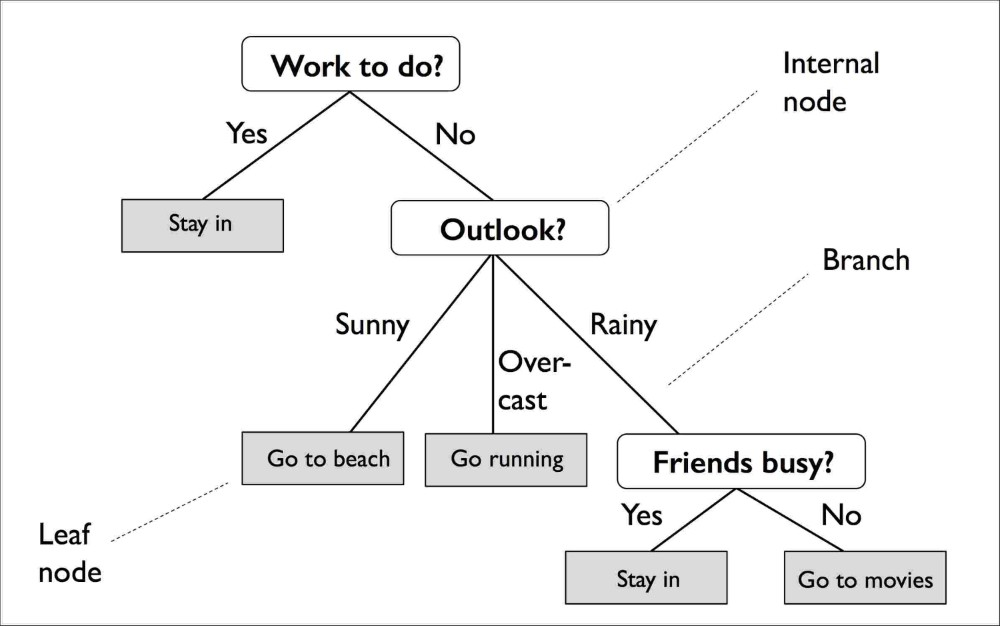
\includegraphics[scale = .55]{imagens/arvore.png}
    \caption{Um exemplo de árvore de decisão. Elaboração própria.}
    \label{fig:arvore}
\end{figure}


\begin{defi}
Seja $\X, \Y$ um par de espaços de mensuração e resposta. Uma \textbf{Árvore de Decisão} é uma função $\A: \X \to \Y$, onde $\Y$ é enumerável, associada à uma árvore $G$. Se $\Y$ for um subconjunto convexo da reta então chamamos de \textbf{Árvore de Regressão}.
\end{defi}

\begin{exemplo}[Regressão]
 Uma empresa de tecnologia no ramo de venda e aluguel de imóveis quer trabalhar em um modelo de precificação de aluguel. A ideia é que donos de imóveis recebam um valor sugerido compatível com o mercado e embutir isso no serviço.
 
 Um analista coletou dados de aluguel e algumas informações básicas do apartamento. Área, número de quartos, de banheiros, se aceita animais, se é mobiliado e em qual cidade está localizado. 
 
 
\end{exemplo}





\section{Noções de Estimação de uma Árvore de Decisão}

Como podemos traduzir uma amostra $A$ em uma árvore de decisão $\A$? Uma abordagem candidata é o procedimento original apresentado na primeira edição de \citeonline{breiman2017classification}.

Imagine que temos uma massa de dados, uma nuvem de pontos em algum espaço de mensuração. 

REESCREVER A PARTIR DAQUI

%Primeiro definimos a \textbf{proporção} de um vértice como um vetor contendo a proporção de cada classe observada nos dados que chegaram ao vértice. Depois, a \textbf{Impureza} do nodo. A função $\I(\cdot)$ mapeia um nodo em um número positivo limitado superiormente por um real $I$ de forma que a impureza de um nodo cuja proporção seja igual para todas as classes seja $0$ e a impureza de um nodo cuja proporção seja unitária para alguma classe seja $I$. Precisamos impor apenas que $\I(\cdot)$ seja monotonamente crescente em relação à probabilidade de cada classe. O valor específico da impureza não é relevante, desde que aumente monotonamente em relação à heterogeneidade de proporções observadas.

%Tome uma divisão $D_i$ qualquer. Ela rende duas subamostras/divisões que podem ou não serem terminais, $D_{iA}$ e $D_{iB}$. Defina $P_A (D_i)$ como a proporção de casos que chegam em $D_i$ e vão para $D_{iA}$ e o mesmo para $P_B (D_i)$. A \textbf{Qualidade} da divisão é dada pela variação na impureza: $\mathcal{Q} (D_i) := \I(D_i) - P_A(D_i) \I (D_{iA}) - P_B(D_i) \I (D_{iB})$.


%Note que a qualidade é uma variável aleatória. O processo de formar uma árvore de decisão a partir de um certo conjunto de dados é chamado de treinar a árvore. Escolher a divisão adequada envolve muitos recursos computacionais e selecionar a divisão que maximize a qualidade dentre as potenciais. Qualquer regra computável pode ser usada: um valor ser maior ou menor que um certo patamar, estar em uma certa faixa, etc. Os aspectos algorítmicos deste problema são interessantes porém fogem ao escopo desta monografia, discussões podem ser encontradas em \citeonline{de1991distance}.
 
 \section{Construindo uma Floresta Aleatória}
 
 A agregação das predições de árvores construídas a partir de pedaços diferentes da amostra é um passo seguinte e natural à modelagem anteriormente apresentada. Como os procedimentos de escolha de divisões são estocásticos, árvores individuais de decisão podem apresentar vieses ou baixa performance ao acaso. Se um número grande de árvores é agregado e não há relação sistemática do erro de predição com alguma variável preditiva, então os erros devem se anular com o aumento do número de árvores.
 
 %\begin{defi}
 %Seja $A$ uma instância de um Banco $(\mathcal{X}, \C)$. Existe um conjunto de subamostras únicas dessa instância, $B = \{ B_1, B_2, ..., B_k\}$  independentes. Treine em cada elemento de $B$ uma árvore de decisão $\A_i$ e chame de $F(x)$ o conjunto de imagens obtidas ao aplicar cada $\A_i$ a uma observação $x$ da instância $A$. Uma \textbf{Floresta Aleatória} é um classificador $\F : F(x) \to \C$. 
  %\end{defi}
  
  %\begin{defi}
 % Seja $A$ uma instância de um Banco $(\mathcal{X}, \C)$ com $n$ observações. Seja $F$ um conjunto de $k$ árvores de decisão treinadas em $A$ de acordo com a definição anterior. Seja $x_i$ a $i$-ésima observação da instância $A$ e, por fim, $\1(\cdot)$ a função indicadora. A \textbf{Margem} da floresta aleatória $\F$ formada pelas árvores de decisão $\A_j$ na observação $x_i$ é a função $M(\F, x_i) := \sum_{j=1}^k \1 ( \A_j (x_i) = \C(x_i) ) - \sum_{j=1}^k \1  ( \A_j (x_i) \neq \C(x_i) )$.
 % \end{defi}
  
 
 % \begin{defi}
 %Para uma observação $x$ de uma instância $A$, o \textbf{Erro de Generalização} $G(\F, x) := \Prob (M(\F, A, x)) < 0)$.  \end{defi}
  
 % A margem provê uma medida do quão precisa é a floresta em votar corretamente na classe verdadeira da observação. Uma margem maior sinaliza uma maior capacidade da floresta de discriminar o dado observado entre possíveis classes.  

 %\begin{teo}[Convergência do Erro de Generalização] Seja $A$ uma instância de um Banco $(\mathcal{X}, \C)$. Defina a sequência $E_k = \{ G(\F_k, A, x) \}$ de forma que $\F_k = \F_{k-1} \bigcup \A_k $,  Tome as classes possíveis $\C = \{1,2,3,...,c,...,J \}$ e uma observação $x$, tal que $\C(x) = c$. Então $E_k \to \sum_{i=1}^k \1 ( \A_i (x) = c ) - \underset{}{\text{Max}} \sum_{i=1}^k \1  ( \A_i (x) \neq c) $
 
% \end{teo}
 
Alguns refinamentos muito interessantes podem ser feitos. \textit{Bagging}, a ideia de expor árvores diferentes da floresta à observações e variáveis explicativas diferentes. \textit{Boosting}, treinar uma árvore no resíduo de outra, fazendo a floresta aprender lentamente, incorporando padrões mais sutis. 
 
 
 
 \begin{prova}
 Ver o Apêndice 1 de \citeonline{breiman2001random}. \blacksquare
 \end{prova}


\chapter{Econometria Clássica e Efeitos Marginais}

Introduzido o conceito de Floresta Aleatória, agora voltamos nossa atenção à Econometria Clássica e seu  modelo central. Veremos uma maneira de estimar os parâmetros desse modelo via Mínimos Quadrados Ordinários, como modelos de Floresta Aleatória não têm a mesma interpretabilidade e como podemos contornar essa problemática avaliando o modelo na vizinhança de algumas observações. A apresentação seguirá \citeonline{hayashi}. 



\section{Teoria Clássica de Regressão Linear}

Retornando um pouco, e apenas esse pouco, ao capítulo anterior, usaremos de novo os conceitos de variáveis explicativas (que aqui chamaremos de \textbf{regressores}) e de uma variável resposta. Suponha que observamos $n$ medidas. Então $y_i$ é a $i$-ésima observação da variável resposta e o vetor $(x_{i1}, x_{i2}, ..., x_{ik})$ a $i$-ésima observação dos $k$ regressores. Quando nos referimos a um modelo aqui, estamos nos referindo ao conjunto de restrições sobre a distribuição conjunta dos regressores e da resposta. A Teoria Clássica de Regressão Linear se apoia nas Hipóteses 1-4 a seguir.

\begin{hipotese}[Linearidade]
Nossos modelos têm a seguinte forma funcional, onde $\beta_j$ são os parâmetros a serem estimados e $\epsilon_i$ é o termo que chamamos de \textbf{resíduo}. 


\begin{align}
    y_i = \sum_{j = 1}^k \beta_j x_{ij} + \epsilon_i \label{mod_lin};
\end{align}

Linearidade implica que o efeito de uma variação em um regressor particular na resposta não depende do seu nível, nem do de outros regressores. De fato:

\begin{align}
    \frac{\partial y_i}{\partial x_{ij}} = \beta_j
\end{align}
\end{hipotese}


O modelador pode usar de intuição para construir variáveis novas que são funções não-lineares das variáveis mensuradas originalmente. A relação entre salário e experiência ou escolaridade, por exemplo, tem retornos decrescentes. Os primeiros cinco anos no mercado de trabalho contribuem muito mais para um aumento salarial do que os últimos cinco anos de carreira. Essa relação pode ser captada introduzindo um termo com o quadrado da experiência no modelo ou uma variável discreta valendo $1$ nos primeiros anos de carreira e $0$ depois, por exemplo. 


Antes de prosseguir é importante apresentar a notação matricial dos modelos lineares. Uma maneira interessante de nos referir aos dados coletados de uma amostra - e como discutiremos estimação isso é importante - é associa-los à uma matriz. Notaremos uma \textbf{matriz de dados} como $\mathbf{X}$, preenchida com a $i$-ésima observação da $j$-ésima variável. Também teremos $\mathbf{y}$, o vetor em que a $i$-ésima entrada é a medida da variável resposta da $i$-ésima observação, e $\mathbf{\epsilon}$, o vetor com o resíduo. Finalmente, os parâmetros $\beta_j$ estarão no vetor $\boldsymbol{\beta}$. A partir de agora usaremos $n$ para nos referir ao tamanho da amostra, o número de linhas em $\mathbf{X}$ e $\mathbf{y}$. Reescrevendo a equação \ref{mod_lin} em notação matricial:

\begin{equation}
    \underset{n \times 1}{\mathbf{y}} = \underset{n \times k}{\mathbf{X}} \,\, \underset{k \times 1}{\boldsymbol{\beta}}   + \underset{n \times 1}{\boldsymbol{\epsilon}} .
\end{equation}



\begin{hipotese}[Exogeneidade Estrita]
A média condicional do erro é nula.

\begin{align}
    \E[\epsilon_i \, | \, \mathbf{X}] = 0;
\end{align}

Essa hipótese não é restritiva se, entre as variáveis explicativas, houver uma com valor constante igual à média incondicional dos resíduos do modelo sem o valor constante. É assim de trás para frente que encontraremos o intercepto do modelo no processo de estimação, inclusive. 

\end{hipotese}

\begin{hipotese}[Ausência de Multicolinearidade]
O posto da matriz de dados $\mathbf{X}_{n \times k}$ é $k$ com probabilidade 1.
\end{hipotese}

Em termos práticos, supomos que as variáveis dadas para um modelo linear são linearmente independentes umas das outras. Se os valores de uma variável podem ser inteiramente determinados por combinações lineares de outras, qualquer informação que possa trazer já está contida nas outras. Também supomos que nosso modelo erra de maneira consistente:

\begin{hipotese}[Homocedasticidade]
Seja $\E$ o operador de esperança:

\begin{align}
    \E[\epsilon_i^2\, |\, \mathbf{X} ] = \sigma^2;
\end{align}

A variância dos resíduos independe do nível dos regressores.

\end{hipotese}

\begin{exemplo}[Heterocedasticidade]
É simples violar a hipótese 4, basta tornar o componente não-observado uma função de alguma variável explicativa. Adicionando esse comportamento no processo simulado temos:

\begin{figure}[H]
    \centering
    
    \captionbox{Uma amostra simulada do processo.}{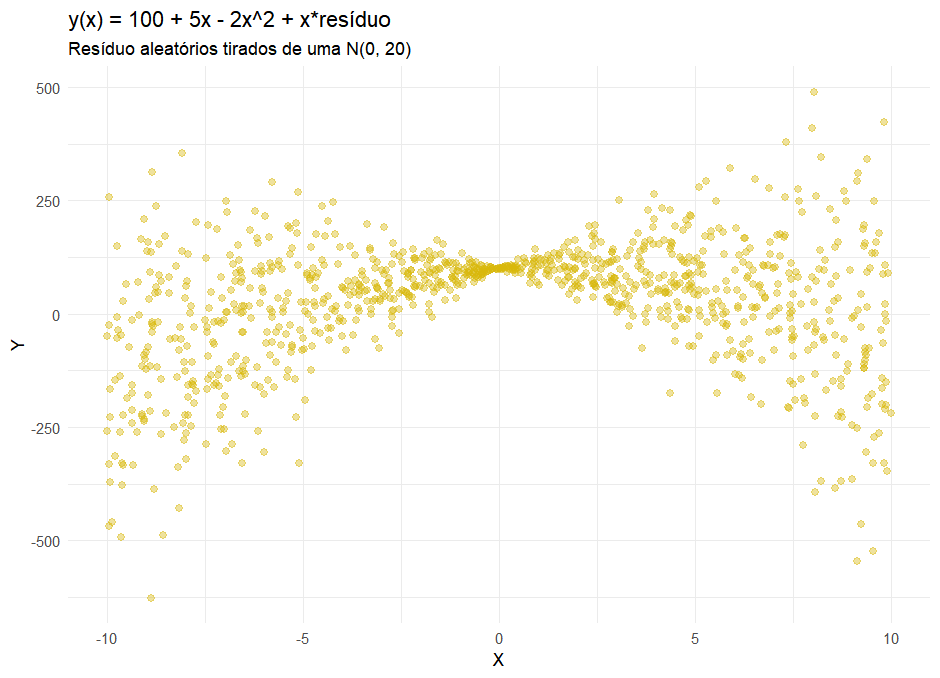
\includegraphics[scale = .75]{imagens/exemplo_heteroske.png}}
    \fonte{Elaboração própria.}
\end{figure}

\begin{table}

\caption{\label{tab:tabela_hetero}Modelo com termo quadrático. Elaboração própria.}
\centering
\begin{tabular}[t]{l|r|r|r}
\hline
termo & estimativa & erro\_padrao & estatistica\_t\\
\hline
(Intercept) & 97.64 & 6.97 & 14.01\\
\hline
x & 24.72 & 3.15 & 7.86\\
\hline
x2 & -2.37 & 0.30 & -7.95\\
\hline
\end{tabular}
\end{table}


Agora quando tentamos recuperar os parâmetros obtemos estimativas estatisticamente significantes, como informa a Tabela \ref{tab:tabela_hetero}. Os parâmetros estimados, no entanto, estão à dezenas de desvios-padrão dos verdadeiros, como mostramos na Figura 6.


\end{exemplo}



% Dadas as Condições de Gauss-Markov e uma amostra $(\mathbf{X}, \mathbf{y})$, se $(\mathbf{x}_i, \mathbf{y}_i)$ são i.i.d vale que $ \E[\epsilon_i^2\, |\, \mathbf{X} ] = \E[\epsilon_i^2\, |\, \mathbf{x}_i ]  $.


\section{Efeitos Marginais}
\subsection{Em Modelos Lineares}
A primeira hipótese, Linearidade, é a chave aqui. A resposta, supomos, varia linearmente nos regressores. Podemos introduzir algumas interações criando variáveis novas que são funções não-lineares das variáveis originais, adicionamos logaritmos, potências, indicadoras e outras tantas transformações para acomodar não-linearidades. Essa abordagem promissora, no entanto, necessariamente diminui a precisão da estimativa de todos os parâmetros e seus graus de liberdade, impondo restrições.

Mesmo que essa perda de precisão seja tolerável, esbarramos em um problema embutido na construção desses modelos. Estimamos um escalar para descrever o efeito marginal de uma variável sobre a resposta e apenas isso. Estamos supondo por definição que os efeitos marginais são iguais em todo o suporte e para qualquer nível dos outros regressores. Essa hipótese, no entanto, não está presente em florestas aleatórias.

\subsection{Em Florestas Aleatórias}

Suponha que temos uma árvore treinada $\A$ e uma observação $x$. Com alguma licença poética nos referimos à previsão dessa árvore para essa obervação como $\A(x)$. De maior incômodo para o econometrista é que não é claro o que exatamente é a derivada dessa função. Isso é um problema porque boa parte da utilidade de um modelo (linear) estimado é ter um vetor de parâmetros intuitivamente interpretáveis, pois contém as derivadas parciais do modelo. 

A derivada de $\A(\cdot)$, seja lá como for, não é tão informativa. Uma pertubação em uma observação $x$ só altera o resultado da previsão de uma árvore se for grande o suficiente para deslocar $x$ para outra regra de classificação/previsão. Teríamos uma função que é nula em boa parte de seu domínio, descontínua onde não for. 

O problema é atenuado com uma floresta aleatória. Uma pertubação pequena em $x$ pode alterar a previsão de uma fração das árvores da florestas. Com um número suficientemente grande de árvores uma variação arbitrariamente pequena em $x$ leva à uma variação arbitrariamente pequena em $\F(x)$ e vale alguma forma de continuidade. 

Esse caminho sugere uma estratégia promissora. Podemos perturbar uma observação de referência e as previsões de seus vizinhos. Isso gera uma curva relacionando valores de um regressor, dado um vetor níveis para os outros regressores, às previsões. Sua inclinação nos dá os efeitos marginais, que ao contrário do que acontece em modelos lineares, são sensíveis aos níveis dos regressores que não estamos perturbando.

\section{Um Procedimento de Computação}

Suponha um modelo $\M : \X \to \Y$. Como computamos seus efeitos marginais de maneira agnóstica? Gostaríamos de aplicar um mesmo procedimento e identificar os efeitos marginais sem depender da mecânica particular de uma classe de modelos. Por trás dos panos cada classe opera um maquinário completamente diferente: redes neurais são composições sucessivas de transformações lineares, modelos lineares são polinômios, máquinas de vetores de suporte calculam distâncias de vetores a um hiperplano estimado com base nos dados. 

Se as mecânicas internas de $\M$ variam demais para termos um procedimento uniforme, podemos olhar onde não há variação entre classes de modelos, $\X$ e $\Y$. Observando os valores que as predições do modelo dão para a resposta $Y$ em uma curva parametrizada $t \in \X$ basta computar a sua derivada para achar os efeitos marginais na curva. 

Como normalmente estamos interessados no efeito de tratamento individual de uma variável, talvez seu efeito conjunto com outra, o problema é limitado a avaliar o modelo ao longo de uma ou duas dimensões apenas. Avaliar o efeito marginal de mais variáveis implica apenas repetir o procedimento, não sofrer da maldição da dimensionalidade. Esse procedimento é computacionalmente simples, barato e agnóstico ao modelo.



\chapter{Aplicação do Procedimento}

Neste capítulo o procedimento será ilustrado em um modelo de regressão de preços de imóveis. Os dados foram adquiridas via \textit{webscrapping} de um site nacional de aluguel de imóveis para 4 capitais brasileiras no dia 20 de Março de 2020, realizado pelo autor. Iremos estimar uma série de modelos com variadas configurações de hiperparametros e computar algumas métricas de sucesso para explorar como eles afetam performance do modelo. Essas métricas de sucesso serão computadas com dados omitidos no processo de treinamento, num processo chamado Validação Cruzada, e então aplicaremos o procedimento descrito no capítulo anterior.

\section{Otimização de Hiperparametros}

Não existe uma única maneira de estimar uma floresta aleatória. De fato, como machine learning é um campo que cresceu muito às margens da academia, em laboratórios da indústria, as convenções são informais e há pouco escrito em pedra. Optei por usar a implementação em \citeonline{ranger}, que usa como gatilho de geração de folhas uma amostra abaixo da mínima chegar no nodo e aleatoriza quantas variáveis explicativas são usadas em cada árvore. Uma alternativa de alta confiabilidade seria \citeonline{randomForest}. Para a otimização de hiperparametros, validação cruzada e avaliação dos modelos foi usada a plataforma \texttt{tidymodels} \cite{tidymodels}, implementada em linguagem R \cite{R}.

Decidida a implementação que irá realizar as computações, é preciso fazer uma escolha sobre os hiperparâmetros do modelo, no caso três: amostra mínima para criação de folha, número de árvores e número de variáveis a serem aleatoriamente escolhidas para cada árvore. Do ponto de vista do expectador desinteressado o problema é apenas:

\begin{align}
    \mathbf{x}^* = \underset{\mathbf{x}}{\text{arg max}} \,\,\phi(\mathbf{x}) 
\end{align}

E como seria fácil se soubéssemos exatamente o que é $\phi(\cdot)$, mas não sabemos. Uma primeira abordagem é tatear o suporte da função em busca da melhor combinação. Um método para isso é \textit{random search}, gerar algumas combinações de hiperparâmetros aleatórias, estimar um modelo em cada e escolher o de melhor performance, que definiremos em detalhes brevemente. O dual dessa abordagem é \textit{grid search} em que ao invés de gerar combinações aleatórias se cobre o espaço de hiperparâmetros de vetores com distância regular, gerando uma grade. 

Essas são ditas abordagens \textbf{caixa-preta livre de modelo} pois não fazem suposições sobre a forma funcional da função a ser maximizada ajustando os hiperparâmetros. Varremos o que acreditamos ser o seu domínio à força bruta. Existem alternativas. \citeonline{shahriari2015taking} é um tratamento amplo da principal, otimização bayesiana. Otimização de Hiperparâmetros é um campo grande. Um tratamento mais detalhado do estado da arte na área está disponível em \citeonline{feurer2019hyperparameter}.


\begin{figure}[H]
    \centering
    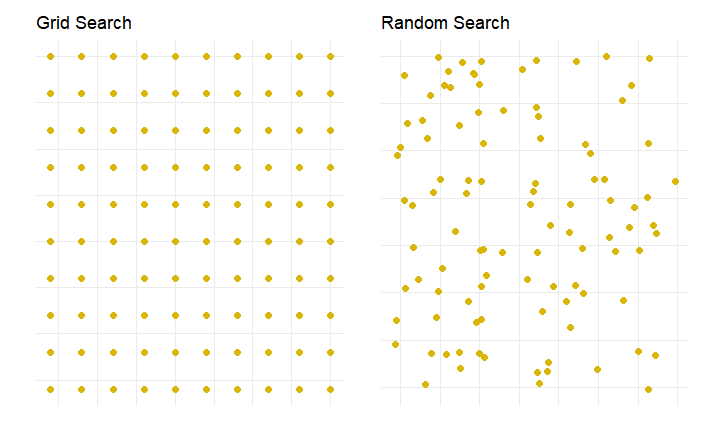
\includegraphics[scale = .75]{imagens/random_grid.png}
    \caption{Duas buscas de 100 modelos cada. Elaboração própria.}
\end{figure}

\section{Métricas de Qualidade}

Na seção anterior optamos por escolher hiperparâmetros de forma a maximizar alguma função que entendemos ser algo como a ''qualidade'' de um modelo. Precisamos agora definir como computa-la. Métricas de performance de modelo são sempre arbitrárias então a boa prática recomenda usar uma cesta delas. As opções para regressão são inúmeras. Serão avaliadas seis:

\begin{itemize}
    \item \textbf{Razão Performance-Interquatil (RPIQ)} \newline
    Definida como o desvio-padrão das previsões dividido pela amplitude interquartil da resposta. Mede principalmente a consistência do modelo, não a acurácia preditiva. Quanto mais próximo de 1, melhor. 
    
    \item \textbf{Coeficiente de Concordância de Correlação (CCC)} \newline
    Introduzido por \citeonline{lawrence1989concordance}, mede tanto consistência quanto acurácia. Calculada a partir da diferença entre a identidade e a reta de regressão dos valores preditos nos verdadeiros. Quanto mais próximo de 1, melhor.
    
    \item \textbf{Erro Médio Absoluto (MAE)} \newline
    A média das diferenças entre previsões e valores verdadeiros. Diretamente interpretável na unidade original da resposta. Indica acurácia. Menor é melhor, mas deve-se atentar à parcimônia.
    
    \item \textbf{Erro Médio Percentual (MPE)} \newline
    A média das diferenças entre previsões e valores verdadeiros ponderada pela média da resposta. Lida em unidades relativas. Indica acurácia. Menor é melhor, mas deve-se atentar à parcimônia.
    
    \item \textbf{Coeficiente de Determinação (R2)} \newline
    Calcula-se a soma dos quadrados dos desvios das previsões à média da resposta. Dividi-se esse valor pela soma dos quadrados dos desvios as observações originais à média da resposta. O resultado está entre $0$ e $1$ e pode ser interpretado como a fração da variância que o modelo consegue explicar. Mede principalmente consistência, não acurácia. Maior é melhor, mas deve-se atentar à parcimônia pois cresce monotonamente no número de variáveis explicativas.
    
    \item \textbf{Raiz do Erro Quadrático Médio (RMSE)} \newline
    O Erro Quadrático Médio é a média dos quadrados dos desvios das previsões em relação aos valores verdadeiros. A raiz dá a métrica. Mede principalmente acurácia, embora seja muito sensível a outliers. Menor é melhor.
    
\end{itemize}

Em um contexto de classificação precisamos de outras métricas. A título de exmeplo, algumas das mais amplamente utilizadas são:

\begin{itemize}
    \item \textbf{Sensitividade/ Recall} \newline
    Em classificação binária, a Sensitividade é a proporção dos casos positivos que são corretamente identificados.
    \item \textbf{Especificidade} \newline
    Em classificação binária, a Especificidade é a proporção dos casos negativos que são corretamente identificados.
    \item \textbf{Acurácia} \newline
    A fração de casos corretamente identificados. 
    \item \textbf{Precisão/ Valor Preditivo Positivo} \newline
    O número de verdadeiros positivos dividido pelo número de preditos positivos.
    \item \textbf{F1-Score} \newline
    Média harmônia da Precisão e da Sensitividade
    
\end{itemize}


\section{Validação Cruzada}

Para dar uma chance melhor a cada combinação podemos testa-la em amostras diferentes. Fazemos isso com validação $k$-cruzada. Dividimos a amostra em $k$ grupos aproximadamente iguais e para cada combinação de hiperparâmetros estimamos o modelo em $k-1$ combinações, excluindo um grupo de cada vez. Como medida de performance para cada combinação específica de hiperparâmetros usamos então a média das métricas de performance nas $k-1$ validações. 

Um pouco de sabedoria popular com florestas aleatórias sugere que o número de árvores não é um bom hiperparâmetro para se validar. Os ganhos de performance são pequenos, o custo computacional, no entanto, variante. Note que o custo de estimar uma floresta cresce linearmente, um para um, com o número de árvores. Validar $k$ combinações cada uma com $a*b$ árvores é $a$ vezes mais caro que validar $k$ combinações com $b$ árvores. 

Esse tempo de computação é melhor empregado procurando com uma grade fina melhores combinações de amostra única e número de variáveis por árvore. Árvores com menos variáveis tem menos variância, o que ajuda a diminuir a variância da floresta, e menor poder preditivo. Árvores com menor amostra mínima têm mais folhas, criando respostas mais finas, mas têm mais variância também. 


\begin{figure}[H]
    \centering
    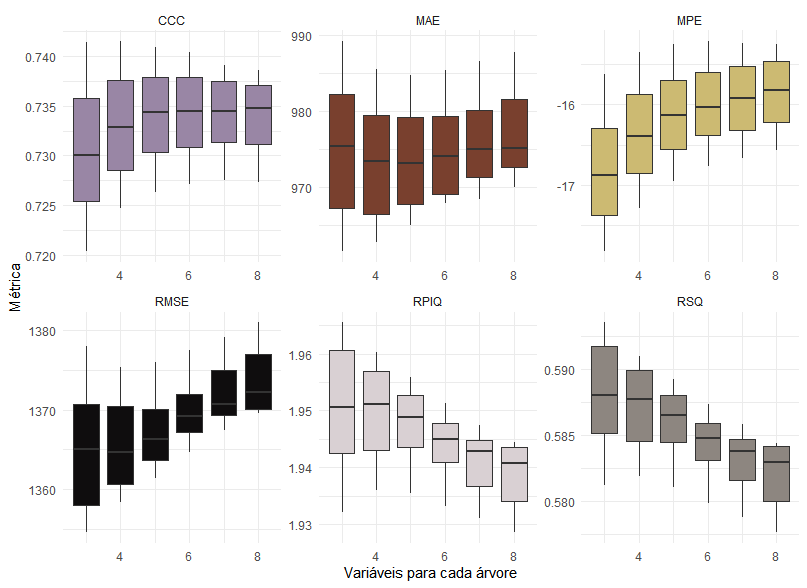
\includegraphics[scale = .72]{imagens/cross_v_mtry.png}
    \caption{Resumo de métricas de performance variando quantas variáveis alimentar para cada árvore. Elaboração própria.}
\end{figure}

Percorrendo o domínio de números de variáveis possíveis e mapeando o efeito em algumas métricas de performance vemos que nesse contexto esse hiperparâmetro não parece muito relevante, embora exista sim variação de performance. Ela, no entanto, não é consistente entre as métricas. Podemos, e devemos, verificar o que ocorre variando o tamanho de uma amostra que gatilha a geração de uma folha contendo uma regra de previsão/classificação. 


\begin{figure}[H]
    \centering
    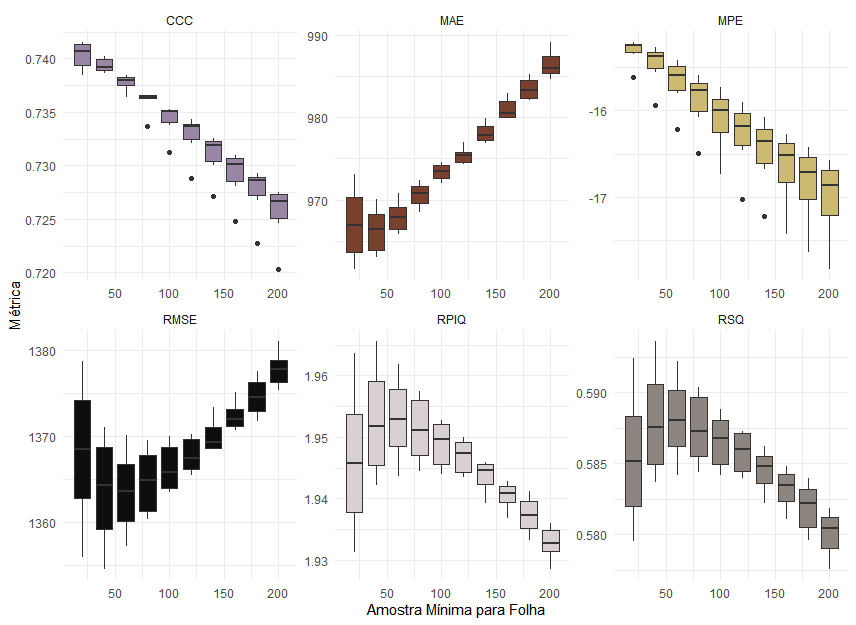
\includegraphics[scale = .70]{imagens/crossv_min.png}
    \caption{Resumo de métricas de performance variando a amostra mínima para criar uma folha. Elaboração própria.}
\end{figure}


Variando a amostra mínima para geração de folhas vemos mais variação nas métricas de performance. Amostras mínimas maiores geram menos regras de previsão/classificação distintas e portanto aumentam erros de previsão mais ou menos monotonamente. Ocorre concavidade com métricas como RPIQ, R2 e RMSE, todas similares e com picos em torno de 60 observações. 

E afinal qual seria o ''melhor'' modelo? A Regra do Um Desvio \cite{breiman1984classification} sugere escolher o modelo mais simples que esteja em até um desvio-padrão da performance do melhor modelo. Aplicando essa heurística em cada métrica temos seis sugestões distintas e melhor modelo:

\begin{table}[H]

\caption{\label{tab:tabela_metricas}Melhor modelo de acordo com cada métrica. Elaboração Própria.}
\centering
\begin{tabular}[t]{c|c|c}
\hline
Variáveis por Árvore & Amostra Mínima para Folha & metrica\\
\hline
3 & 20 & RPIQ\\
\hline
4 & 20 & CCC\\
\hline
3 & 20 & MAE\\
\hline
3 & 200 & MPE\\
\hline
3 & 20 & RSQ\\
\hline
3 & 20 & RMSE\\
\hline
\end{tabular}
\end{table}




\section{Computação de Efeitos Marginais}

\begin{figure}[H]
    \centering
    \includegraphics[scale = .70]{imagens/efeitos_marginais_rf.png}
    \caption{ Elaboração própria.}
\end{figure}



\begin{figure}[H]
    \centering
    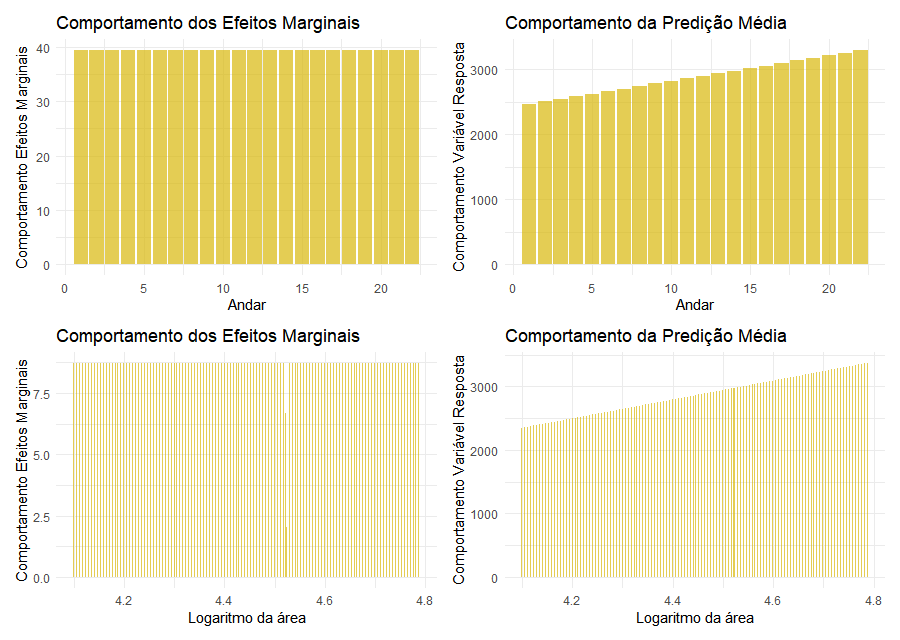
\includegraphics[scale = .70]{imagens/efeitos_marginais_lm.png}
    \caption{ Elaboração própria.}
\end{figure}
\input{capitulos/cap5.tex}
%% ------------------------------------------------------------------
% Aqui, o objetivo é mostrar como colocar uma imagem ou um gráfico 
% na presente monografia. tudo que faremos é usar um ambiente 
% gráfico e assim, iremos o gerar. 
%-------------------------------------------------------------------

%-------------------------------------------------------------------
% Novamente, para preenchermos o documento, usaremos o lipsum
%-------------------------------------------------------------------

\chapter{Conceitos Matemáticos}
Esta monografia está permeada de argumentos matemáticos formais, de fato é a sua contribuição central. Como os requisitos matemáticos ao seu entendimento são um tanto quanto específicos, aqui faço uma breve exposição da teoria necessária ao entendimento com um grau adequado de rigor. Tratamentos mais ou menos rigorosos existem em abundância e as duas principais referências são \cite{rudin} e \cite{pugh}.

Alguns cuidados com definir apropriadamente corpos, operações de soma e multiplicação foram omitidos. É do meu entendimento que uma concepção operacional não-rigorosa destes conceitos é suficiente para os propósitos desta monografia.

Dividi essa seção em quatro partes. Em \ref{primeira} cubro alguns aspectos básicos como métricas e sequências, culminando na demonstração de que o $(\mathbb{R}^k, d)$ é um espaço métrico completo se $d(.,.)$ for uma métrica plena. Em \ref{segunda} abordamos Topologia Ponto-a-Conjunto com um grande enfoque nos reais. O fato central que esta seção trará será o teorema de Bolzano-Weierstrass. As ferramentas descobertas nessa seção serão de enorme uso ao longo de toda esta monografia. Em \ref{terceira} abordaremos funções e alguns resultados de teoria de ponto fixo. Na \ref{quarta} concluímos este pequeno curso relâmpago ao abordar espaços de funções e equações diferenciais.


\section{Sequências, Espaços Métricos e Completude}
\label{primeira}


\subsection{Métricas}

Uma discussão interessante sobre processos estocásticos requer uma bem definida noção de distância. Afinal, o que faz dois elementos \textit{distarem} um do outro e como mediremos isso? Imagine um conjunto $X$ como quiser. Um disco, os reais, um contorno de pato no plano cartesiano... 

\begin{defi}
Uma \textbf{métrica} é uma função $d: X \times X \to \mathbb{R}$ que atende quatro propriedades:

\begin{itemize}
    \item \textbf{Simetria:} $d(x,y) = d(y,x)$. 
    \item \textbf{Unicidade:} $d(x,x) = 0$.
    \item \textbf{Positividade:} $d(x,y) \geq 0$
    \item \textbf{Desigualdade Triangular:} $d(x,y) \leq d(x,z) + d(z,y)$. 

\end{itemize}
\end{defi}

Observe que as três primeiras propriedades que estamos exigindo de uma métrica apenas formalizam nossa intuição sobre como distâncias se comportam no mundo real. Ir de um lugar ao outro deve cobrir a mesma distância que a volta se usarmos a mesma rota. A distância de um ponto até ele mesmo é nula (quanto você, leitor, precisa andar para ficar parado?) e distâncias negativas seriam coisas no mínimo curiosas.

A Desigualdade Triangular é definitivamente a propriedade mais interessante de uma métrica. Ela essencialmente diz que não existem "atalhos" em um contexto em que existem distâncias. A distância entre dois pontos quaisquer sempre é no mínimo a mesma que a soma das distâncias entre estes mesmos pontos e um terceiro. Em um contexto de plano cartesiano este fato é rapidamente visualizado com a ajuda de um triângulo. 

\begin{center}
\tikzset{every picture/.style={line width=0.75pt}} %set default line width to 0.75pt        

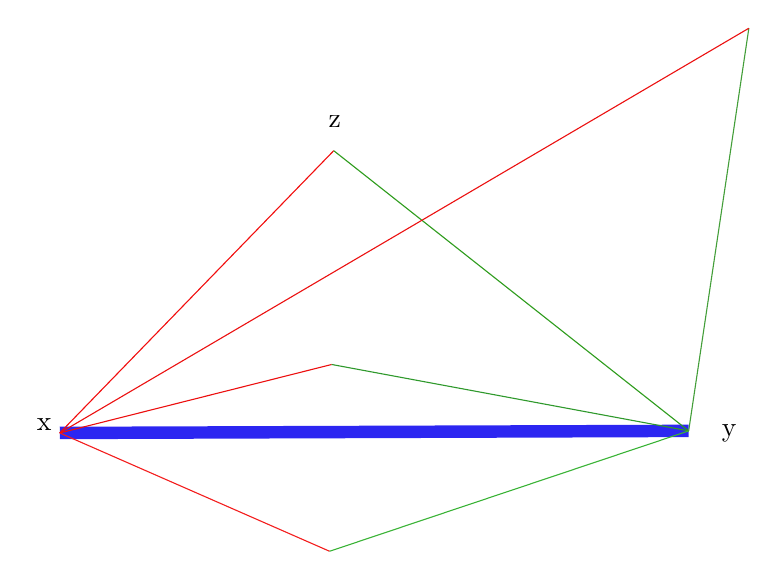
\begin{tikzpicture}[x=0.75pt,y=0.75pt,yscale=-1,xscale=1]
%uncomment if require: \path (0,300); %set diagram left start at 0, and has height of 300

%Straight Lines [id:da6847309088840179] 
\draw [color={rgb, 255:red, 44; green, 38; blue, 241 }  ,draw opacity=1 ][line width=4.5]    (69.5,214) -- (372.5,213) ;


%Straight Lines [id:da46426148005512835] 
\draw [color={rgb, 255:red, 241; green, 13; blue, 13 }  ,draw opacity=1 ]   (201.5,78) -- (69.5,214) ;


%Straight Lines [id:da2906024541588399] 
\draw [color={rgb, 255:red, 46; green, 156; blue, 29 }  ,draw opacity=1 ]   (201.5,78) -- (372.5,213) ;


%Straight Lines [id:da6028165286195768] 
\draw [color={rgb, 255:red, 236; green, 15; blue, 15 }  ,draw opacity=1 ]   (69.5,214) -- (200.5,181) ;


%Straight Lines [id:da6610711832317098] 
\draw [color={rgb, 255:red, 47; green, 153; blue, 44 }  ,draw opacity=1 ]   (200.5,181) -- (372.5,213) ;


%Straight Lines [id:da7902181564457826] 
\draw [color={rgb, 255:red, 243; green, 29; blue, 29 }  ,draw opacity=1 ]   (69.5,214) -- (199.5,271) ;


%Straight Lines [id:da8016282193076851] 
\draw [color={rgb, 255:red, 58; green, 179; blue, 54 }  ,draw opacity=1 ]   (372.5,213) -- (199.5,271) ;


%Straight Lines [id:da6023664239656019] 
\draw [color={rgb, 255:red, 67; green, 158; blue, 57 }  ,draw opacity=1 ]   (401.5,19) -- (372.5,213) ;


%Straight Lines [id:da5175708881441581] 
\draw [color={rgb, 255:red, 235; green, 17; blue, 17 }  ,draw opacity=1 ]   (401.5,19) -- (69.5,214) ;



% Text Node
\draw (62,210) node  [align=left] {x};
% Text Node
\draw (392,214) node  [align=left] {y};
% Text Node
\draw (202,64) node  [align=left] {z};


\end{tikzpicture}
\label{desitri}
\end{center}




Na figura \ref{desitri} a desigualdade triangular é clara. Em qualquer um dos triângulos, a soma do comprimento das arestas vermelha e verde é sempre menor que a azul. Existem variadas métricas, apresento aqui alguns exemplos:

\begin{itemize}
    \item \textbf{Métrica Euclidiana:} $d(x,y) = \sqrt{\sum_{i=1}^k (x_i - y_i)^2}$. Esta é a noção usual de distância que temos. Com esta métrica, o menor trajeto entre dois pontos sempre é uma reta. Observe que em uma dimensão a métrica euclidiana é simplesmente $x-y$. Em duas é o tamanho da hipotenusa do triângulo retângulo inscrito nos dois pontos. Em três é o tamanho da diagonal do cubo inscrito nos pontos e por aí vai.
    \item \textbf{Métrica Discreta:} $d(x,y) = \mathbb{1}(x \neq y)$. Uma noção um pouco curiosa de distância em que se dois elementos são diferentes dizemos que distam uma unidade. 
    \item \textbf{Métrica "Taxista":} $d(x,y) = \sqrt{\sum_{i=1}^d (x_i - y_i)}$
\end{itemize}



\subsection{Espaços Métricos}

\begin{defi}
Um \textbf{Espaço Métrico} é uma dupla de um conjunto $X$ e uma métrica $d$. Nos referimos ao espaço munido deste ambiente e dessa noção de distância como $(X,d)$.
\end{defi}

Esse conceito é mais fino e amplo do que parece à primeira vista. Estamos falando de conjuntos, então meras coleções de elementos, e de métricas, maneiras de medir distâncias. Digamos que estamos no plano cartesiano. Um conjunto qualquer prontamente se torna um espaço métrico ao munirmos ele de uma métrica - Euclidiana, discreta ou que for - e agora ganhamos espaço de manobra para garantir que certos fenômenos ocorram nele.

O poder de pensar em termos de Espaços Métricos com tanta generalidade é que conseguimos ver com mais clareza o que há de comum entre o plano cartesiano e a superfície arredondada da terra - e como espaços diferentes podem por vezes pedir métricas diferentes para responderem problemas de ordem mais prática. Conceber distância como a reta que liga dois pontos faz muito sentido no plano cartesiano ou no $\mathbb{R}^k$, mas nem tanto ao falar da superfície da terra, em que normalmente modelamos a distância entre dois pontos como o menor arco na superfície que ligue-os. 




\subsection{Sequências e Limites}


\begin{defi}
Uma \textbf{sequência} $x:\mathbb{N} \to \mathbb{R}^k$ é uma função que mapeia os naturais em elementos de algum conjunto. Podemos, alternativamente, entender uma sequência como um conjunto $\{x_n\} = \{ x_n \in \mathbb{R}^k \,\, | \,\, n \in \mathbb{N}\}$. Dizemos que uma sequência tem \textbf{limite} em $L$ - alternativamente que $L$ é limite de $x_n$ ou que $x_n$ \textbf{converge} a $L$ - se $\forall \,\, \epsilon > 0 \,\, \exists \,\, n' \in \mathbb{N} \,\, | \,\, n > n' \implies d(x_n, L) < \epsilon$. Notamos $\lim_{n \to \infty} x_n = L$
\end{defi}

Sequências são apenas conjuntos de elementos com um processo definidor. Imagine por exemplo a sequência contida na reta real $x_n = \frac{1}{n}$, ou uma prima não-muito-distante contida no $\mathbb{R}^2$, $y_n = (\frac{1}{n}, \frac{10}{n})$. Observe que $\lim x_n = 0$ e que $\lim y_n = (0,0)$. Podemos construir uma infinidade de outros exemplos, seguem alguns - todos com a métrica euclidiana em mente.

\begin{itemize}
    \item $x_n = (1 + \frac{1}{n})$ \implies 
    $\lim x_n = 1$ 
    \item $x_n = (1, 2n, \frac{79}{n})$ \implies
    $\lim x_n = (1, \infty, 0)$
    \item $x_n = \sin{n}$ \implies
    $\nexists \lim x_n$
    \item $x_n = (1+\frac{1}{n})^n$ \implies $\lim x_n = e$
    \item $x_n = (-\frac{4n^2}{3n}, n, \pi)$ \implies $\lim x_n = (-\infty, \infty, \pi)$
    \item $x_n = 2$ \implies $\lim x_n = 2$
\end{itemize}


Aos nos referir a números arbitrariamente pequenos como $\epsilon > 0$ estamos tão somente dizendo que não importa o quão arbitrariamente próximo de um ponto limite quer-se chegar, se uma sequência converge a este limite, existe algum índice natural tal que a sequência está à uma distância menor que $\epsilon$ deste limite. Observe que não importando qual natural seja escolhido, a rigor, $\frac{1}{n}$ jamais será de fato igual a zero e sim à grandezas arbitrariamente pequenas. No entanto, dada uma distância arbitrária do zero, sempre podemos atingi-la com este sequência que tenha limite em zero ao escolher um $n$ suficientemente grande. Esta é a noção de limite.

Talvez agora comece a fazer um pouco mais de sentido a escolha deliberada de falar com generalidade de distâncias. $x_n = 1/n$ por exemplo tem limite em $0$ na métrica euclidiana, mas na discreta não.

\subsection{Sequências de Cauchy}

Temos agora um pequeno problema teórico em mãos. A depender da métrica, algumas sequências cujos termos se aproximam arbitrariamente de certos pontos podem ou não ter limites. Como lidamos com isso? Abriremos mão da noção de limite e focaremos no comportamento em si: termos de uma sequência que estão cada vez menos distantes entre si.

\begin{defi}
Uma sequência é \textbf{de Cauchy} se $\forall \,\, \epsilon > 0 \,\, \exists \,\, n \in \mathbb{N} \,\, | \,\, a,b > n \implies d(x_a,x_b) < \epsilon$.
\end{defi}

Uma sequência de Cauchy apresenta essa propriedade de que para qualquer distância arbitrária de $0$ que se escolha, existe algum ponto a partir do qual todos os termos da sequência distam no máximo essa distância arbitrária, por menor que seja. Uma sequência de Cauchy é, no português mais direto, uma em que os termos subsequentes estão sempre cada vez mais próximos.

Essa noção pode ser difícil de diferenciar de uma sequência que tem limite em algum ponto então façamos um pequeno exercício mental. Imagine que estamos no espaço métrico $(\mathbb{Q}, d)$. Imagine agora a seguinte sequência:

$$a_1 = 3$$
$$a_2 = 3,1$$
$$a_3 = 3,14$$
$$a_4 = 3,141$$
$$a_5 = 3,1415$$
$$a_6 = 3,14159$$
$$...$$
$$a_{30} = 3,1415926535 8979323846 2643383279$$
$$...$$

Eu espero que seja claro ao leitor que essa sequência $a_n$ é de Cauchy. O que não pode parecer claro a princípio é que, apesar disso, não existe limite para essa sequência. Isto porque ela se aproxima arbitrariamente de $\pi$ e estamos no espaço métrico $(\mathbb{Q}, d)$. Esta sequência está indo \textbf{para fora} do espaço -  porque $\pi$ é um número irracional - ainda que seja de Cauchy e tenha termos cada vez mais próximos uns dos outros. 

\subsection{Espaços Métricos Completos}

Note que se descrevermos uma sequência de Cauchy em um espaço que esteja se aproximando de um elemento desse mesmo espaço, ela necessariamente converge, temos um limite. Será então que existem espaços em que \textbf{toda} sequência de Cauchy converge? Já sabemos que isso claramente não procede para espaços $(\mathbb{Q}, d)$, qualquer que seja a métrica.

Voltemos ao exemplo da sequência $a_n$ que se aproximava de $\pi$. Se fizermos uma operação de "colar" esse buraco faltando nos reais, a história muda. Imagine o conjunto $A = \mathbb{Q} \bigcup \{\pi\}$. Se estivermos no espaço $(A,d)$ então $\exists \lim a_n$ e mais ainda, $\lim a_n = \pi$. Isso nos deixa agora com outra infinidade de sequências que são de Cauchy e não convergem no espaço $(A,d)$ porque se aproximam arbitrariamente de números irracionais como $e$ e $\sqrt{2}$. Repetindo a operação de colar os irracionais até que tenhamos colado todos faz com que $A = \mathbb{Q} \bigcup \mathbb{I}$. 

Perceba que a união dos racionais com os irracionais dá o conjunto dos números reais e que por construção qualquer sequência de Cauchy em um espaço $(\mathbb{Q} \bigcup \mathbb{I}, d)$ converge. É impossível construir uma sequência de Cauchy de números reais que não tenha como limite outro número real. Em um espaço métrico construído com números reais, \textbf{toda} sequência de Cauchy converge. Este fato é notável e merece uma conceitualização própria.

\begin{defi}
Um espaço métrico $(X,d)$ é \textbf{completo} se nele toda sequência de Cauchy converge.
\end{defi}

Os Reais caracterizam um espaço métrico completo. Ao contrário do que ocorre nos Irracionais e nos Racionais, ambos permeados de "buracos". Completude é uma propriedade muito interessante de espaços métricos e veremos mais à frente que ela é central para a validade de alguns teoremas extremamente úteis como o do Ponto Fixo de Banach. 

Recapitulando, começamos esta seção falando de métricas. Apenas formalizamos nossa intuição sobre o que significam distâncias. A partir daí construímos um novo conceito, o de sequências e vimos que sequências são maneiras de nos aproximarmos de números de maneiras arbitrárias. Vimos depois que a depender de qual conjunto usamos para construir nossos espaços métricos, se aproximar arbitrariamente de um ponto não quer dizer convergir a ele. Por isso refinamos nosso conceito de sequência e conhecemos as sequências de Cauchy. Logo uma pergunta absolutamente natural emergiu. Queríamos saber se existem espaços em que ter um limite e ser uma sequência de Cauchy são sinônimos. Por serem "especiais" nesse sentido, demos a eles um nome específico: espaços métricos completos. E assim o são por não terem os "buracos" que racionais e irracionais têm.

Agora voltamos nossas miras para a topologia elementar ponto-a-conjunto, onde estudaremos as propriedades mais gerais de conjuntos e de espaços. 

\section{Topologia Ponto-a-Conjunto Elementar}
\label{segunda}




\subsection{Interioridade e Abertura}
\subsection{Vizinhanças e Bolas}
\subsection{Aderência e Proximidade}
\subsection{Limitação e Compacidade}
\subsection{Teorema de Bolzano-Weierstrass}


\section{Funções, Continuidade e Pontos Fixos}
\label{terceira}
\subsection{Mapa, função, transformação, campo ou correspondência?}
\subsection{Compacidade e Continuidade}
\subsection{Homeomorfismos, Retrações, Contrações e outras formas de deformar espaços}
\subsection{Um brevíssimo passeio pelos Teoremas de Ponto Fixo}
\subsubsection{Os Teoremas de Brouwer e Kakutani: Deformando Conjuntos Convexos}
\subsubsection{O Teorema do Ponto Fixo de Banach: Contraindo Espaços Completos}



\section{Mapeando Espaços de Funções}
\label{quarta}
\subsection{Espaços de Funções}
\subsection{Equações Diferenciais como Mapas do Espaço de Funções}
\subsection{Equações em Diferenças e Mapas Iterados}


\chapter{Processos Estocásticos}

Aqui faço uma exposição breve, autocontida e razoavelmente formal do objeto central deste estudo.


\begin{defi}

Um \textbf{Processo Estocástico n-dimensional} é uma sequência  $\{X_t\}_{t \in T} \subset \Omega \subseteq \mathbb{R}^n$ onde $X_t$ é uma variável aleatória e o conjunto $T = \{1,2,...,t\}$ indexa a passagem do tempo.  
\end{defi}

Confrontados com dados do mundo real, observamos apenas \textbf{uma} realização particular do processo qualquer que comande o fenômeno estudado. Logo, ao descrever a realização do processo como uma sequência, ela necessariamente caracterizará um subconjunto próprio do espaço amostral $\Omega$. 

\section{Processos Autoregressivos}

%-------------------------------------------------------------------
% O que faremos abaixo é incluir uma imagem (formato JPG, mas 
% poderia ser outro formato) no pdf. O argumento width=\textwidth 
% ajusta a largura da imagem a largura da página
%-------------------------------------------------------------------

%\begin{figure}[h]
%	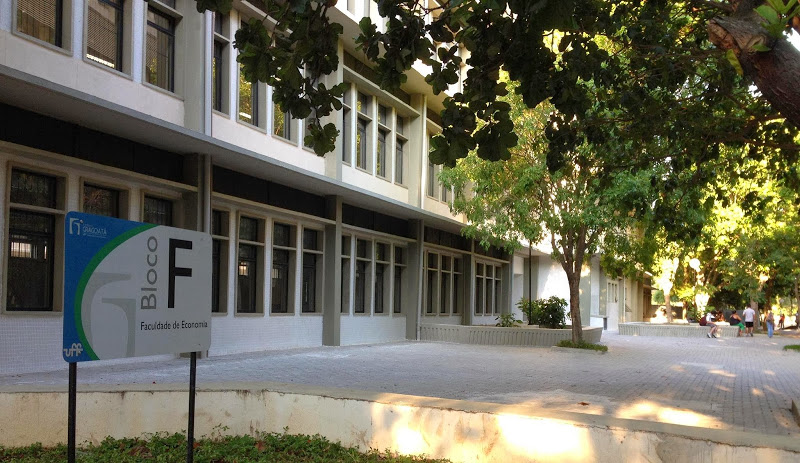
\includegraphics[width=\textwidth%]{imagens/blocof.jpg}
%	\caption{O Bloco F}
%	\label{fig:blocof} % Aqui %'nomeamos' o gráfico
%\end{figure}

%-------------------------------------------------------------------
% mais lipsum...
%-------------------------------------------------------------------


%-------------------------------------------------------------------
% Aqui mostraremos, por fim, como realizar uma citação
%-------------------------------------------------------------------

\chapter{Como Citar}
\label{cap:cite}

Supondo que desejássemos realizar uma citação no texto, por exemplo do pacote que usamos para fazer esse modelo de monografia. Tudo que teríamos que fazer seria utilizar o comando \texttt{citeonline\{\}} ou o \texttt{cite\{\}}. Usando o ambiente de citação, teríamos abaixo o exemplo.\cite{osbourne2009ozzy}

\begin{citacao}
	``Exemplo de um ambiente de citação. Não usamos o comando \texttt{citeonline\{\}}. Então, ao fim do ambiente iremos usar, entre parênteses para simular uma citação em ABNT.'' 
\end{citacao}


\chapter{Conclusões}
\label{cap:conclusoes}

Foi demonstrado como construir uma floresta aleatória partindo de primeiros princípios. Depois, através de notação matricial clássica no campo, como e o que são modelos lineares. A problemática de estimar efeitos marginais foi apresentada e um procedimento computacionalmente simples para isso em seguida, demonstrando como algumas nuances passavam batido por modelos lineares.

O tema é relevante em dois sentidos. Do ponto de vista do aprendizado de máquina, porque encaixa em uma agenda maior de pesquisa em \textit{interpretabilidade} de Machine Learning. O núcleo duro reduzido da disciplina abre espaço para uma série de más práticas disseminadas no uso dessas técnicas \cite{flach2019performance}. Avaliar efeitos marginais pode ser usado como uma forma de validação qualitativa também. Relações com sinais inversos ao esperado podem ser sinal de problemas.

Há também, pelo mesmo motivo, dificuldade de comunicação de resultados de modelos e até mesmo responsabilização civil-criminal quanto às consequências de seu uso em ambiente de produção, sem supervisão humana \cite{lepri2018fair}. Interpretação de modelo, em particular antes de entrega para algum ambiente de produção em que seus resultados afetarão desde experiência de uso em aplicativos de jogos à possivelmente investigação criminal, é crucial. O economista se preocupa com interpretabilidade porque é, de certa maneira, a finalidade principal do trabalho aplicado de métodos quantitativos. Estimar efeitos marginais, (semi)elasticidades e grandezas similares representa a esmagadora maioria das aplicações de econometria, salvo raros estudos como \citeonline{edison2020text} que usam técnicas não-supervisionadas vindas de Linguística Computacional.

Uma limitação não-resolvida da técnica é a inferência dos efeitos marginais computados. É possível distingui-los estatisticamente de zero com algum teste de hipótese? Isso equivale a estabelecer uma ponte entre as duas culturas de \citeonline{breiman2001statistical}. Não parece um problema intratável. Se florestas aleatórias têm distribuição normal e estimamos várias, então temos dados e podemos fazer inferência se conhecermos a variância da floresta. Não é um problema trivial, mas está ao alcance da pesquisa. Essa avenida de pesquisa é provavelmente a de maior interesse ao econometrista aplicado e parte diretamente dos princípios elaborados nesta monografia.









% ----------------------------------------------------------
% ELEMENTOS PÓS-TEXTUAIS
% ----------------------------------------------------------
\postextual

% ----------------------------------------------------------
% Referências bibliográficas
% ----------------------------------------------------------

\nocite{abntexmanual, 
		abntex2modelo} % aqui citamos os autores que não foram citados no texto.

\bibliography{referencias}


\end{document}
